\section{Public good accumulation --- a model,  and potential relevance to Y. pestis}

Matt Asker, Lluis Hernandez and Mauro Mobilia work in the field of antimicrobial resistance \cite{asker2023coexistence}.    Cancerous cells exhibit two varieties: those resistant to a drug, and those succeptible. The resistant ones produce a substnce which they expell into their surrouning matrix. It's called a public good because it facillitates the resistance of all cancer cells to the drug, both the resistant and suceptible types. \par 
It occured to me that there may be something similar going on with Y. pestis in macrophages. -- This is purely my speculation, and may not at all be the case, but even if it isn't, the dynamics may be interesting in and of themselves.  -- Y. pestis has evolved resistance to the toxins that are presented within macrophages.  It occured to me that if Y. pestis were to execute this resistance using a "public good" substance,  that it would be confined within the resident macrophage and thus concentrated, rather than being dispersed.  Something like this could further support the argument that the within-macrophage environment provides a replicative advanage (assuming there are also toxins and other challenge factors (possibly bacteriophages) in the extracellular space). 


\begin{figure}[H]
    \centering
   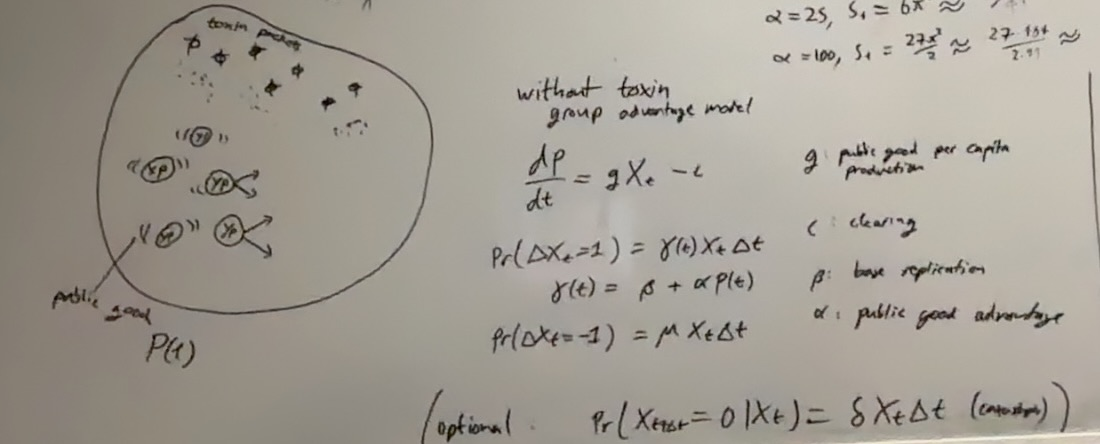
\includegraphics[width=0.99\textwidth]{figures/board.jpeg} % Adjust the width as needed
    \caption{Y.  pestis represented within a macrophage along with toxin containing packets.  Public good, $P(t)$ is produced by }
\end{figure}


\subsection*{Model for public good replication without directly accounting for toxic granules}

The effect of the toxic immune substance can be incorporated into the linear death rate.  Of course, this overlooks the dynamics of toxin depletion as discussed in chapter 6,  but it seems good in the interest of simplicity.  And the point of focus is the dynamics of this public good.  Let us make the simplified assumption that the presence of the "public good" increases the replication rate ($P(t)$: public good concentration; $\xt$: Y. pestis bacteria): 


$$\ddt{P} = g \xt - c,$$
$$\pr{\Delta \xt = 1} = \gamma(t)\xt\Delta t + o(\Delta t),$$
$$\gamma(t) = \beta + \alpha P(t),$$
$$\pr{\Delta \xt = -1} = \mu \xt \Delta t.$$

\begin{itemize}
\item[$g$:] public good production rate
\item[$c$:] public good clearing rate
\item[$\beta$:] base birth rate
\item[$\alpha$:] public good advantage
\end{itemize}
It might well make more sense for the presence of public good to reduce the death rate rather than increase the birth rate.  Another formulation could be thought up along these lines. \par 

\subsection*{Potential quantity of interest}

Suppose we consider a successive version of this process for which in the case of late time non-extinction it is assumed that the infected cell dies and infects two more cells.  A simplification which creates a sort of Galton Watson process in which the division probability is subject to embedded dynamics.\par 
In this case,  for the overall GW process to be supercritical,  the probability of within-cell non-extinction must be greater than one half.  We could as the question of what would be the minimum required incident cohort size into a cell to achieve this,  especially in the case where $\mu > \beta$, in which the public good plays a critical role.  In other words, 

$$\text{inf}\{K : \lim_{t\to\infty}\lrb{\pr{\xt > 0 | \xx_0 = K }}\} = \text{?}$$
This could be computed numerically. 


\subsection*{Notes -- public good in a closed group}

What if there is some replication advantage to a cohort of Y. pestis bacteria living within the enclosure of a macrophage; and what if there is something like a public good produced by the bacteria, and confined within the boundary of the host cellular membrane -- this underpinning a benefit of within group (macrophage) cooperative co-existence. \par 

\vspace{10pt}
\noindent
Something that comes to mind is,  as in other cases of cultural practice,  in Jewish communities it has historically been virtuous to cooperate within the community whilst facing outwards with more competitiveness.  In Shakespeare's "The merchant of venice" it is revealed that at the time (16h CE) it was forbidden for Jews to lend money with interest within the community,  whilst being acceptable to do so with Christians. \par

\vspace{10pt}
\noindent
Just like the individual is rewarded -- paid by gains of cooperative advantage - for being effective to the purpose and success of the private group; so the private group can be rewarded for benefiting circles of wider scope.\par 
And going in the other direction, the individual within the individual is crucial in its avarice when chasing personal enterprise. \par 
Surely these things don't need to be contradictory. 



%My feeling is that somewhere in all this is a helathy middle ground between the two extremes of a particular ideological spectrum.  Crudely,  that between the socialist and the individualistic libertarian capitalist.  On the one hand we have everyone driven to povery by the abolition of accute progress; on the other hand, we have the pathology of extreme inequality.  Something in the middle might see a framework of nested groups internally cooperating and externally competing. 



%%%%%%%%%%%%%%%%%%%%%%%%%%%%%%%%%%%%%%%%%%%%%%%%%%%%%%%%%%%%%%%%%%%%%%%%%%%%%%%%%%%%%%%%%%



%%%%%%%%%%%%%%%%%%%%%%%%%%%%%%%%%%%%%%%%%%%%%%%%%%%%%%%%%%%%%%%%%%%%%%%%%%%%%%%%%%%%%%%%%%
